\chapter{Flexibility-based AC-OPF for active network management in distribution grids}
\label{ChapterOPFDSO}
\chaptermark{Flexibility-based AC-OPF for active network management}

\section{Objectives and contributions}

The dynamics of the power system are changing towards a new model where large generators on the high-voltage side of the network are being replaced by smaller generation units placed at the medium-voltage and low-voltage side of the grid. The increasing proliferation of distributed energy resources will have a significant impact on how the distribution network operates. At the distribution level, DERs will give rise to some new operational and planning challenges and, in some cases, problems already solved will rise again. As a result, the increasing number of DERs placed alongside the medium-voltage  and low-voltage distribution networks leads to the need of flexibility services for the DSO. 
This chapter aims to develop an optimization tool for calculating the value and location of the flexibility request that a DSO needs for operating the distribution network and avoid or mitigate network congestions, corresponding to objective $(iv)$ of the thesis research, according to Figure \ref{fig:chapter_obj_iv}. 

\begin{figure}[htbp]
	\centering
	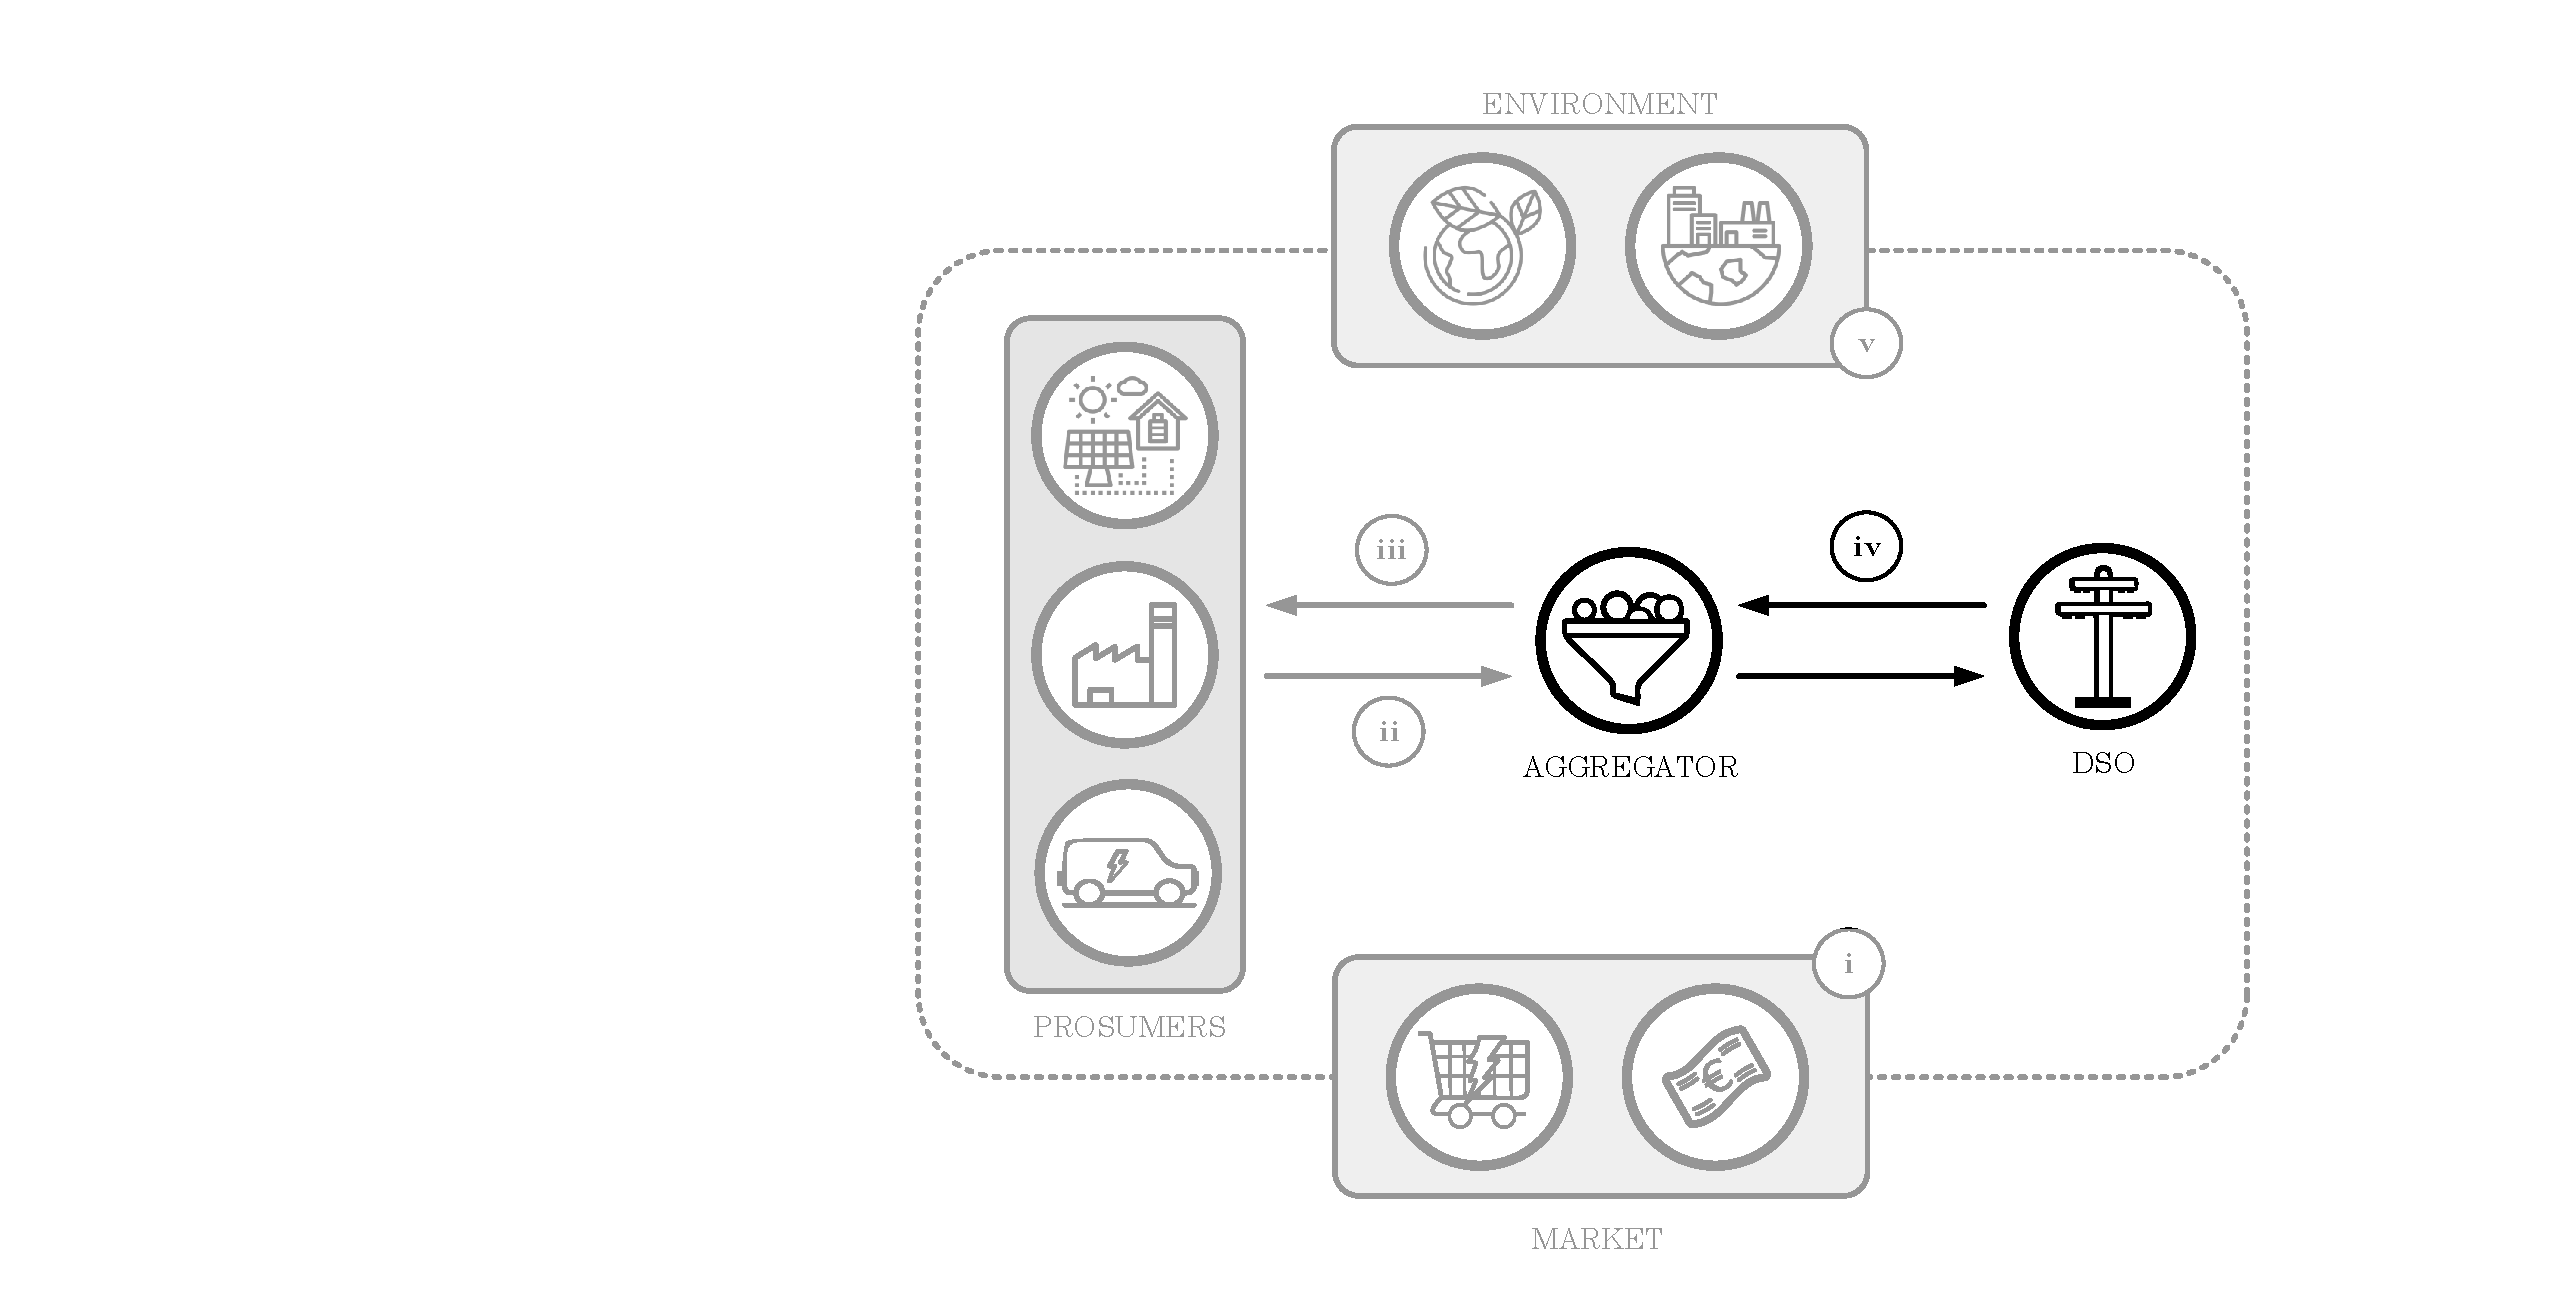
\includegraphics[width=0.7\columnwidth ]{ChapterOPF_DSO/Figures/phd_intro_iv.pdf}
	   %\vspace*{-8cm}
		\caption{Chapter objective based on the PhD scope}
	\label{fig:chapter_obj_iv}  
\end{figure}

These flexibility services could be provided by several demand-side flexible resources such as centralized energy storage, distributed energy storage, electric vehicles, PV panels, or flexible loads such as water boilers or space heaters. The aggregator gathers the flexibility from customers to provide these services to different stakeholders, like energy suppliers, BRPs, TSOs, DSOs, and final consumers \cite{USEFFoundation2015a, Olivella2018}. Then, the aggregator acts as a single entity when engaging in power system markets or selling services to the system operators \cite{BURGER2017}. Under the context of smart grids and flexibility services in place, distribution system operators could benefit by activating flexibility in distribution grids \cite{USEFFoundation2015a, spiliotis2016demand, esmat2016conf, hashemi2016}. First of all, DSOs could compensate grid congestions during high consumption or production periods and therefore reduce the network stress. At the same time, DSOs can increase their renewable generation hosting capacity by using behind-the-meter flexibility during peak production periods. 

The most common problems caused by the high penetration of distributed and renewable generation can be classified into four main categories. Figure \ref{fig:network_problems} provides an overview of the location of these potential problems in an arbitrary distribution network, also detailed in the following list:  

\begin{enumerate}
\item Overload and losses of feeders and transformers. 
\item Voltage deviations (undervoltages and overvoltages).
\item Power quality disturbances.
\item Incorrect operation of protection elements. 
\end{enumerate}

\begin{figure}[h]
	\centering
	\includegraphics[width=1\columnwidth]{ChapterOPF_DSO/Figures/network_problems2.pdf}
	   %\vspace*{-8cm}
		\caption{Distribution network scheme with potential problems and areas}
	\label{fig:network_problems}  
\end{figure}

Based on previous references \cite{ISMAEL20191002, Bollen2011}, the two main potential problems under the distribution network operation are $(i)$ \textbf{overloads} and  $(ii)$ \textbf{voltage deviations}. The following sections defines the potential problems and details the main causes of them. 


\subsection{Overcurrents - Line congestion}
Overloads or commonly also known as overcurrents are those situations where the current circulating through one of the electrical components is higher than the nominal value. This can cause, for example, the damage of the electrical component if the situation happens for a short period of time, the component failure if the current limit is overly exceeded, or additional losses in lines and transformers in the distribution network. However, in many cases, protection elements would trigger and interrupt the service so as to guarantee the correct performance of the component. 
If we consider the current scenario of energy transition with a high penetration of DERs, the risk of overcurrent is mainly caused by the increase of the electricity consumption in a network that has not been reinforced since its construction, and the increase of DERs and electrical appliances such as space heaters, electric vehicles and electric water boilers. In the latter case, the electricity is usually injected at MV and LV levels. Overcurrents happen when the resulting power flow downstream the distributed generator point exceeds the value upstream, under the hyphoteses that no other generation sources are providing energy. This is also related to the feeder capacity limits under normal operation schemes. The scenario where a feeder capacity has been working at its 40-50\% capacity before the integration of capacity generation would have a wider range to allocate these resources than those feeders that in normal operation are at their 90-95 \% of the total capacity. Furthermore, the length of the feeder should be also taken into consideration, since at the beginning of the line the power to be distributed must be equal to the sum of all loads plus the power losses due to the line length, whereas at the end of the feeder only the remaining has to be provided. Hence, the feeder capacity is also related to the length, structure and connected loads. 
Despite the disadvantages and challenges of DERs in distribution networks, it is a fact that DERs can help reduce the losses in the electricity system, since generation is now closer to the consumption points. However, it should be considered that under the case of an excess of generation, reverse flows in MV and LV lines can increase the power losses of the overall system. 

\subsection{Voltage deviations - Undervoltage and overvoltage}
This situation takes place when the voltage value at one or more of the buses is out of the operation rated voltage magnitude, usually $\pm$ 3 \% in LV grids and $\pm$ 2 \% in MV grids \cite{BAYER2020336}. As in the case of overloads, if the overvoltage exceed the upper bound operational constraint, this can lead to the damage of the electrical components and the electric loads connected to that bus. 
For many years, voltage magnitude variations have been a common concern for system operators being the case of undervoltages. This problem is caused by the associated impedance in the distribution lines leading to an excessive voltage droop, but it does not cause any damage to the network components.  

With the increase of DERs integration, utilities have registered an increase of overvoltage cases at the point of common copuling (PCC) of DERs units, and as a result have set up limits on the maximum size of a distributed generator \cite{Kennedy2014}. The reason being that these grid-connected distributed generators do not explicitly regulate voltage, most commonly regulating the active power output. One of the mitigation schemes for overvoltages is the previously mentioned one, establishing restrictions on the distributed generator size and location, under the expansion and planning process of the network. However, with the aim of enhancing the integration of DERs, this could lead to a lack of fairness for end-users who are willing to install DERs at a household or LV-MV level. Another mitigation scheme is the combination of DERs with storage units, avoiding the risk of overvoltage by using the battery to manage the energy surplus. Lastly, DSM techniques and flexibility can help the mitigation of overvoltages in active distribution networks. In the case of undervoltages, DERs can operate under a voltage-reactive power mode with the objective to regulate the reactive power and therefore control the voltage at the connection point, if this is allowed by the network operator \cite{interconnection_ders}. 

\section{Demand-side flexibility for congestion management}
As mentioned in the previous section, the use of demand-side flexibility, managed by aggregators, can help distribution network operators avoid or mitigate congestions. However, as stated in earlier chapters, DSOs and aggregators should be separated entities. DSOs do not have control over the flexible assets for operating the network, and this is the hypothesis on which this chapter is based. This chapter develops a tool for DSOs to calculate the flexibility requests to avoid or mitigate network congestions for a specific time period and under a particular load profile in that network. Therefore, this request will be sent to the aggregator, the entity responsible for providing a service to the network operator and activating the flexibility based on that request. 

Based on the previous assumption where there are specific boundaries between the aggregator and the DSO, a system interaction between these two agents is required to achieve a correct flexibility request interaction. This is depicted in Figure \ref{fig:AGG_DSO_FR}, where the DSO is responsible for calculating their flexibility requests, while the aggregator is the agent receiving these requests, and offers the available flexibility under these conditions of time-horizon and location. If there is a possibility to fulfill the needs of the DSO, then the aggregator is the responsible agent to activate the flexible assets. However, there might be periods where the aggregator cannot cover the totality of the flexibility required. This is why, in all cases, the DSO is the responsible entity to either accept or decline the flexibility offered, being it enough to cover the flexibility required totally or just partially.  

\begin{figure}[h]
	\centering
	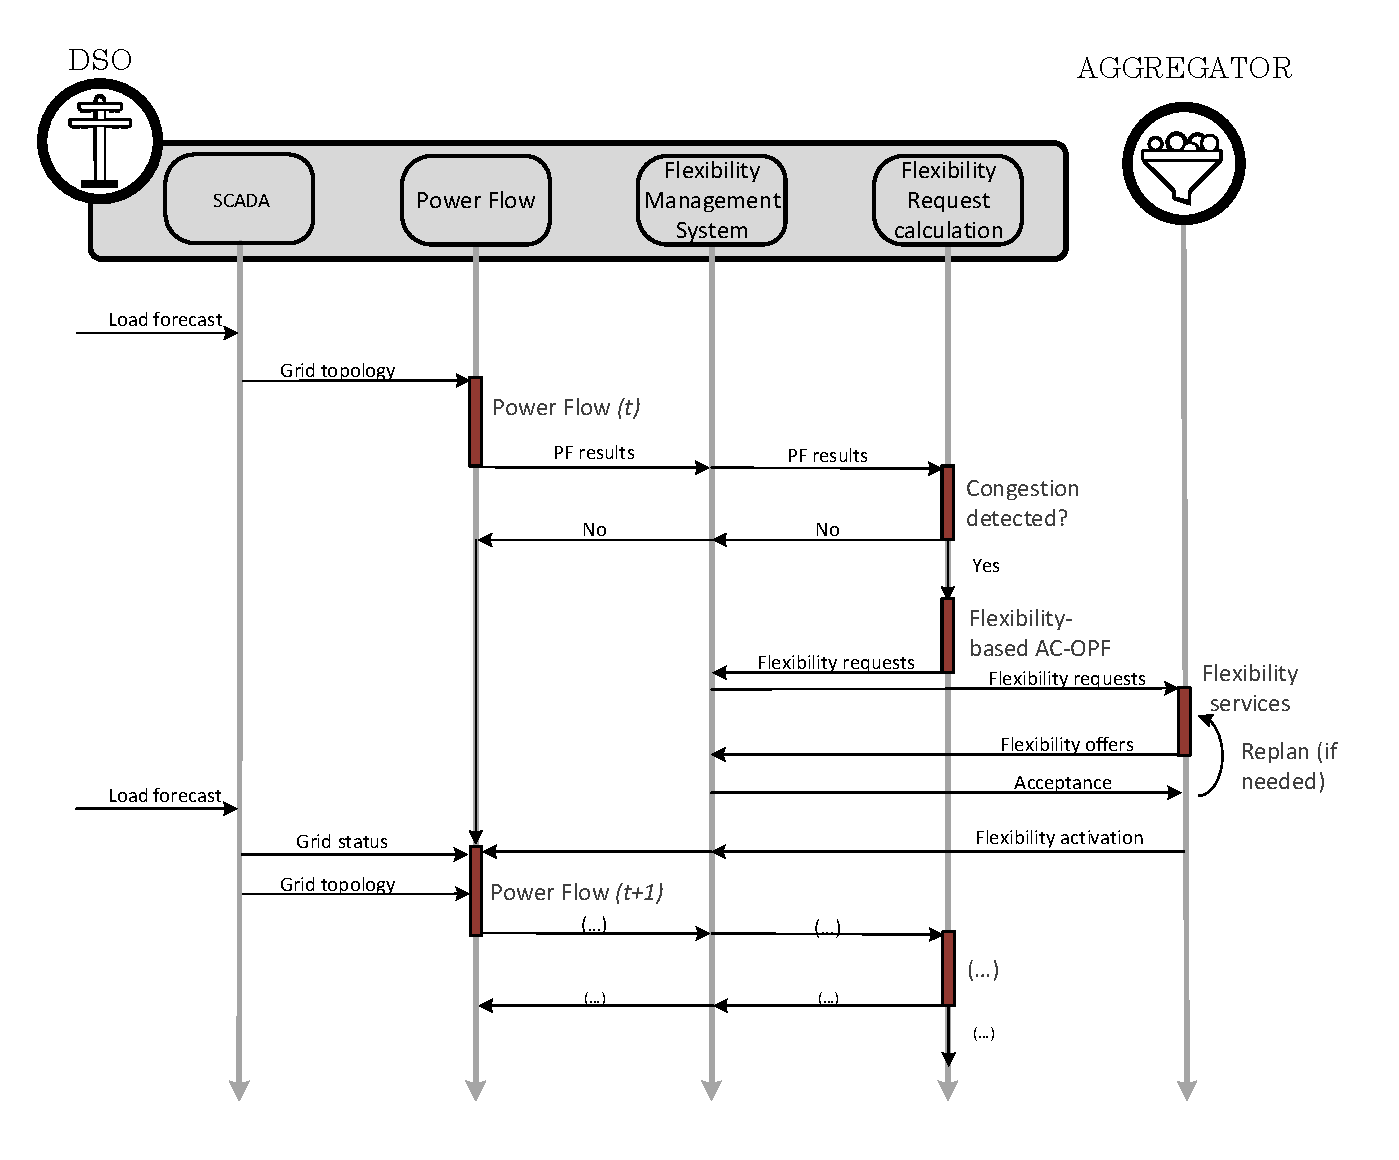
\includegraphics[width=1\columnwidth ]{ChapterOPF_DSO/Figures/OPF_interaction_ACOPF.pdf}
	   %\vspace*{-8cm}
		\caption{Flexibility request interaction}
	\label{fig:AGG_DSO_FR}  
\end{figure}

%\subsection{Standards and protocols for flexibility provision between aggregators and DSOs}
%OPENADR - USEF? 
%\subsection{Literature review on congestion management tools - OPF}
%\subsection{Contribution}
\newpage
\section{Mathematical formulation for flexibility request calculation}
The optimization problem is developed to minimize the aggregator operation costs. The costs are based on curtailing local generation output, charging or discharging batteries, switching off curtailable and disconnectable loads and shifting loads during specific time periods. A local flexibility market design is presented in [12], described as a market-based mechanism for aggregators. BRP and DSO are the main stakeholders of these flexibility services and they can buy flexibility from a market platform or a bilateral contract. However, in any case an information exchange is required between the flexibility buyer and the flexibility provider, to agree on the quantity and delivery time of this flexibility to be provided. 


The problem to solve is mainly an alternating current optimal power flow (AC-OPF), considering as the objective function the minimization of the total flexibility activation costs, also considering the distribution network related constraints. The following section outlines the formulation, covering the objective function and the related constraints of the model. AC-OPF formulation is primarily used for optimization of operation and control actions, meaning in the short term horizon. In the recent years, AC-OPF has started to be implemented in local markets, as being the case of study in this chapter, for the procurement of flexibility for the network operator. Contrarily to DC-OPF, AC-OPF considers the full AC power flow equations, becoming a non-convex problem in its original form, and as a result it cannot be guaranteed that the global optimum is found. In a non-convex problem as this case, several local minima can be present. 

This AC-OPF formulation is based on the polar power-voltage formulation \cite{OPF_Formulation}. This formulation represents complex quantities in polar form, and explicitly uses sines and cosines in the power flow constraints. However, in this case the objective function as well as some of the nodal power balance and the power at buses is adapted to the objective of the flexibility provision for DSOs.

This chapter will consider the notation for complex magnitudes by means of module and angle, defining the complex variable with an underline. This can be seen in the voltage value at each of the buses, $\underline{V}_{i,t}$. The polar formulation of this variable can be hence outlined as follows

\begin{equation*}
\underline{V}_{i,t} = V_{i,t} \phase{\theta_{i,t}}
\end{equation*}

Where $V_{i,t}$ represents the voltage module measured in $pu$ for a given node $i \in N$ and time $t \in T$, and $\theta_{i,t}$ the angle in rad. The network topology and the line admittances are represented by the bus admittance matrix, $[Y]_{bus}$. Each element of this matrix is obtained by means of the following equations,

\begin{subequations}
\begin{align*}
& \underline{y}_{bus_{ii}}= \underline{y}_{ik_{sh,1}} + \sum_k \underline{y}_{ik} \\
& \underline{y}_{bus_{ij}} = - \sum \underline{y}_{ij}
\end{align*}
\end{subequations}

Where two different formulations are used depending on the position of the element in the matrix, being $\underline{y}_{bus_{ii}}$ for a diagonal element and $\underline{y}_{bus_{ij}}$ for a non-diagonal element. The subscripts $i$,$k$ and $j$ are buses of the bus network set $N$. The parameters  $\underline{y}_{ik_{sh,1}}, \underline{y}_{ik}$ are obtained from the equivalent $\pi$-model of the network, represented in Figure \ref{fig:pimodel}. In the case of distribution networks with medium and short lines, the shunt elements $\underline{y}_{ik_{sh,1}}, \underline{y}_{ik_{sh,2}}$ should be included on top of the series admittance $\underline{y}_{ik}$. 

\begin{figure}[htbp]
	\centering
	\includegraphics[width=0.7\columnwidth ]{ChapterOPF_DSO/Figures/pimodel4.pdf}
	   %\vspace*{-8cm}
		\caption{$\pi$-model of the network}
	\label{fig:pimodel}  
\end{figure}

In all cases, the relationship between the nodal admittance matrix  $[Y]_{bus}$ and the nodal impedance matrix  $[Z]_{bus}$ is maintained following the following equation 

\begin{equation*}
[Y]_{bus} = [Z]_{bus}^{-1}
\end{equation*}

%represents the shunt admittance element connected at node $i$ required for modeling short and medium lines, being it the case for distribution networks. For the sake of simplicity, we will consider $[Y]_{bus}$ as $[Y]$, being each of the elements in the matrix the i-j element a complex number $\underline{Y}_{bus_ij}$. In the case of distribution networks, being it the case of study in this chapter, the equivalent network scheme in order to obtain the line admittances is based on the $\pi$-model, shown in Figure \ref{fig:pimodel}. This equivalent scheme considers both the series impedance, $\underline{z}_{ik}$, and the shunt admittance $\underline{y}_{ik_1}$ and $\underline{y}_{ik_2}$.

The admittance matrix $[Y]_{bus}$ for a line between nodes $i,k \in N$ can be formulated as a complex formulation, being the $[G]_{bus}$ the real component representing the conductance of the line between nodes $i,k \in N$; and  $[B]_{bus}$ the complex component defined as the line susceptance between nodes $i,k \in N$, both measured in S $[\Omega^{-1}]$. 

\begin{equation*}
[Y]_{bus} = [G]_{bus} + j[B]_{bus}
\end{equation*}

%Where $G_{ik}$ is the conductance of the line and $B_{ik}$ is the susceptance, both measured in S $[\Omega^{-1}]$. $\underline{Y}_{ik}$ belongs to the bus admittance matrix, $[Y]_{bus}$, an $N x N$ matrix, where $N$ is the number of nodes. This matrix is composed by all the nodal admittance of the various buses. It explains the topology and the admittance of the network. It is a symmetric matrix and the way to obtain the elements of this matrix follow the criteria listed below:

%\begin{subequations}
%\begin{align*}
%& \underline{Y}_{bus_{ii}}= \underline{y}_{ik_{1}} + \sum_k \underline{y}_{ik} \\
%& \underline{Y}_{bus_{ij}} = - \sum \underline{y}_{ij}
%\end{align*}
%\end{subequations}

%Where $i$,$k$ and $j$ are buses of the network, and $k$ are all the buses connected to bus $i$. The parameter $\underline{y}_{ik_{1}}$ represents the shunt admittance element connected at node $i$ required for modeling short and medium lines, being it the case for distribution networks. For the sake of simplicity, we will consider $[Y]_{bus}$ as $[Y]$, being each of the elements in the matrix the i-j element a complex number $\underline{Y}_{bus_ij}$. In the case of distribution networks, being it the case of study in this chapter, the equivalent network scheme in order to obtain the line admittances is based on the $\pi$-model, shown in Figure \ref{fig:pimodel}. This equivalent scheme considers both the series impedance, $\underline{z}_{ik}$, and the shunt admittance $\underline{y}_{ik_1}$ and $\underline{y}_{ik_2}$.
%
%\begin{figure}[htbp]
%	\centering
%	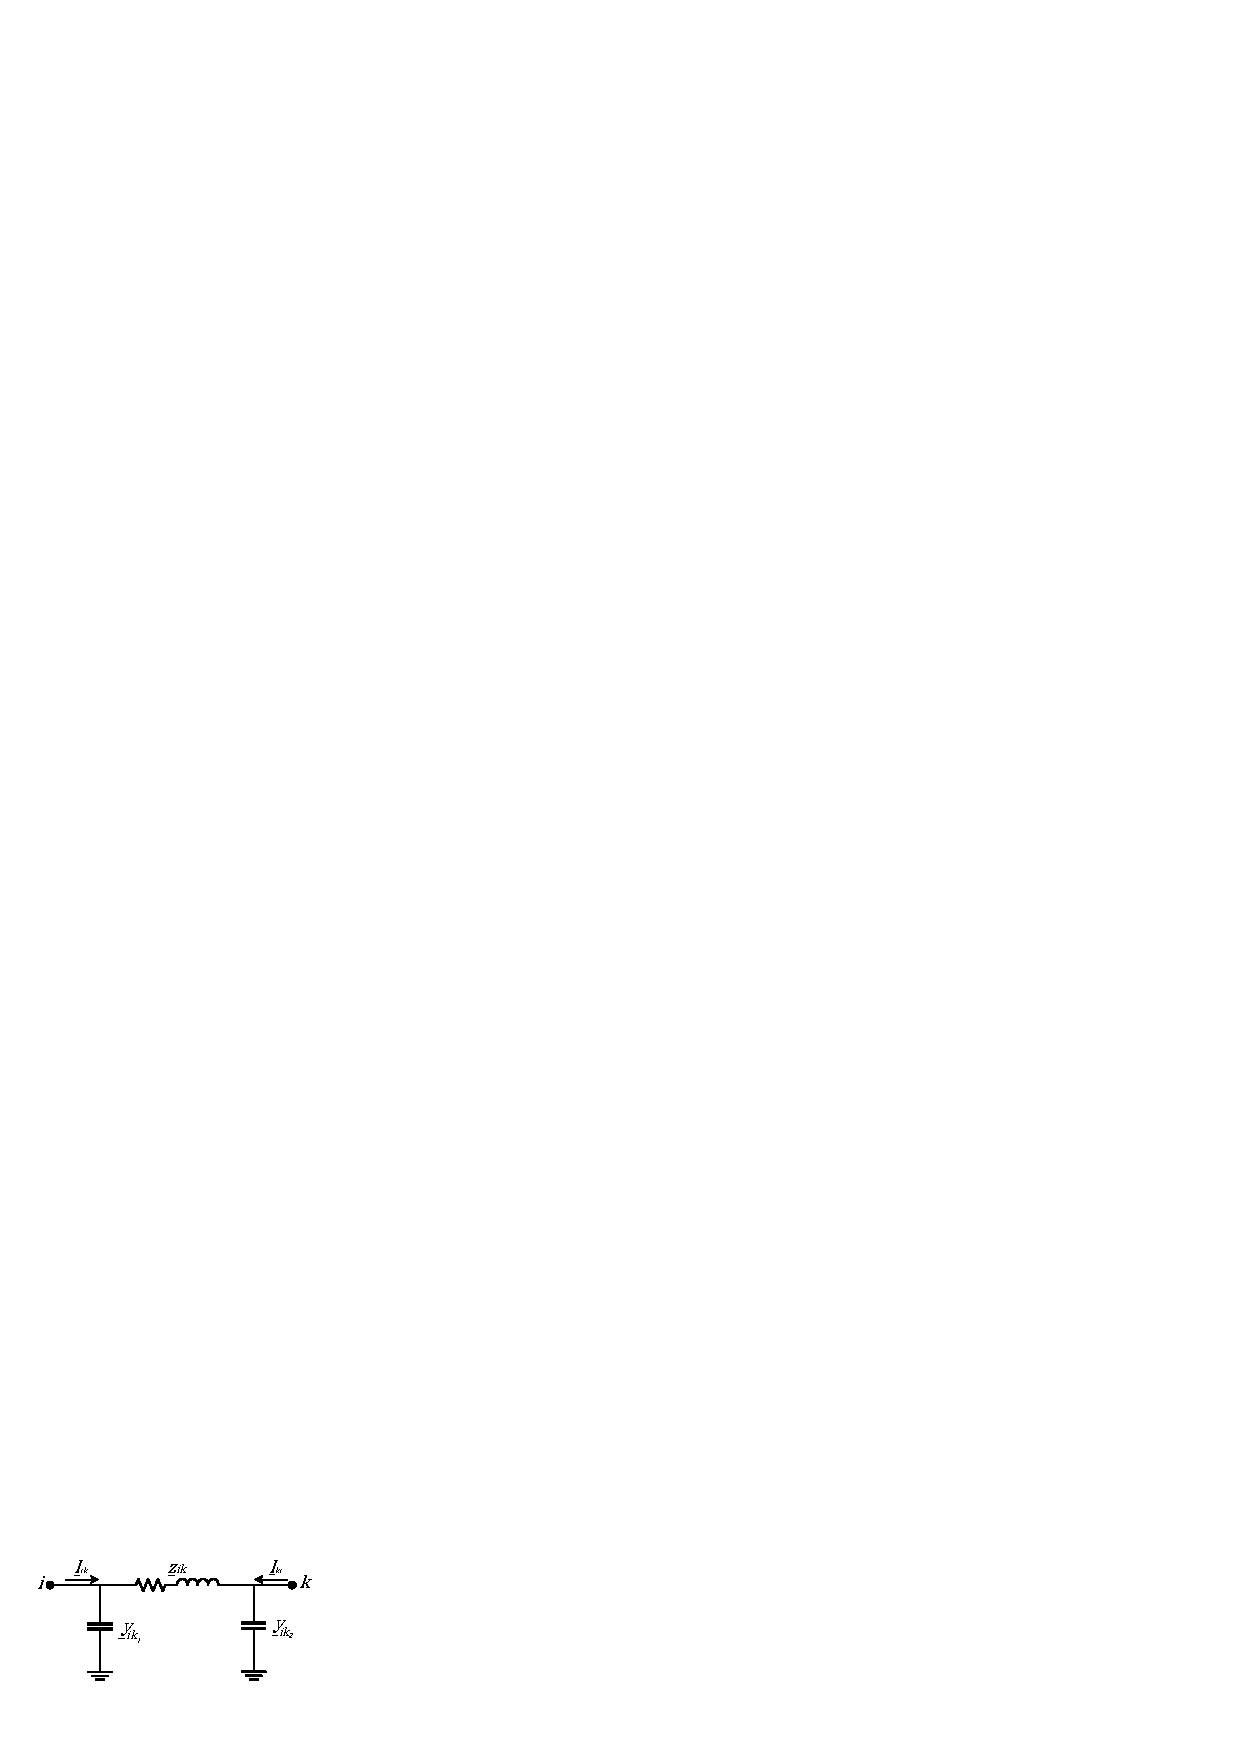
\includegraphics[width=0.7\columnwidth ]{ChapterOPF_DSO/Figures/pimodel2.pdf}
%	   %\vspace*{-8cm}
%		\caption{$\pi$-model of the network}
%	\label{fig:pimodel}  
%\end{figure}


The apparent power of the bus $i \in N$ and time $t \in T$, $\underline{S}_{i,t}$, measured in kVA, can be decomposed into active, $P_{i,t}$ in kW, and reactive power $Q_{i,t}$ in kvar, by the following equation 

\begin{equation*}
\underline{S}_{i,t} = P_{i,t} + jQ_{i,t}
\end{equation*}

%\subsection{Objective Function}
The objective function is to minimize the total flexibility costs for activating both active and reactive power. This function is based on the flexibility activation price accorded between the aggregator and the DSO for a given time period $t \in T$, $C_t^{P}$, $C_t^{Q}$; measured in \euro/kW and \euro/kvar;  and the total active and reactive power requested, $\phi_{i,t}^{P}$ and $\phi_{i,t}^{Q}$, measured in kW and kvar respectively. This yields

\begin{equation*}
\!\min_{\phi_{i,t}^{P^{UP}},\phi_{i,t}^{P^{DOWN}},\phi_{i,t}^{Q}}  \qquad \sum_{t}^{T} \left( \sum_{i}^{N} C_t^{P} \cdot \phi_{i,t}^{P} + C_t^{Q} \cdot \phi_{i,t}^{Q} \right)  
\end{equation*}

There are a set of constraints involved to ensure the correct calculation of the flexibility request. First of all, in the case of active power, there are two types of flexibility that can be activated, being flexibility upwards, $\phi_{i,t}^{P^{UP}}$, and flexibility downwards, $\phi_{i,t}^{P^{DOWN}}$. These are two of the variables of the optimization problem, for a given node $i \in N$ and time $t \in T$. The two vectors containing all the variables for sets $N$ and $T$ are defined as $\Phi^{P^{UP}}$ and $\Phi^{P^{DOWN}}$. In the case of the reactive power flexibility request variable, it is defined as $\phi_{i,t}^{Q}$, for a given node $i \in N$ and time $t \in T$; being the vector for all nodes $n \in N$ and times $t \in T$ represented as $\Phi^{Q}$.

From the DSO perspective, active power flexibility upwards is meant to be an increase of generation or reduction of consumption, and hence it can be modeled as a generator in a specific node, for a given time period. On the contrary, active power flexibility downwards is meant to be an increase of the load at a specific node location of the network or equally as a reduction of the generation. As a consequence, downwards flexibility can be modeled as a load in a specific network node. When talking about the reactive power flexibility request, no disctintion is made between upwards and downwards, since both generators and loads can provide capacitive and inductive reactive power. 

In terms of considering upwards and downwards flexibility at specific time period and a specific node, there cannot be an active power flexibility request upwards and downwards at the same time. In order to avoid binary variables into the model, the flexibility variables are linked as follows

\begin{subequations}
\begin{align*}
& \phi_{i,t}^{P^{UP}} \cdot \phi_{i,t}^{P^{DOWN}} = 0 & \forall i,\forall t \\
%& \phi_{i,t}^{Q^{UP}} \cdot \phi_{i,t}^{Q^{DOWN}} = 0 & \forall i,\forall t 
\end{align*}
\end{subequations}

In the case of reactive power, since both a generator and a load can provide or consume reactive power, being it considered as inductive or capacitive, the reactive power flexibility request is considered as a single variable $\phi_{i,t}^{Q}$, which can take both positive and negative values. 


The constraints listed below ensure the compliance of the AC power flow equations and a correct system operation. The AC power flow equations describe the power system network operating point in steady state, and are based on complex phasor representation of voltage-current relationship at each node. The active $P_{i,t}$ and reactive $Q_{i,t}$ power flow node balance at node $i \in N$ and period  $t \in T$ are formulated. Similarly, there is an equality constraint to detail the mathematical conversion to express  $\theta_{i,k,t}$ based on the voltage angle at each node. This can be outlined as follows, 

\begin{subequations}
\begin{align*}
& P_{i,t} = V_{i,t} \sum_{k=1}^{N} V_{k,t} (G_{i,k} \cos(\theta_{ik,t}) + B_{i,k} \sin(\theta_{ik,t}) & \forall i,\forall t  \\ 
& Q_{i,t} = V_{i,t} \sum_{k=1}^{N} V_{k,t} (G_{i,k} \sin(\theta_{ik,t}) - B_{i,k} \cos(\theta_{ik,t}) & \forall i,\forall t \\
& \theta_{ik,t} = \theta_{i,t} - \theta_{k,t} 															& \forall i,k \in N, \forall t \\
\end{align*}
\end{subequations}

The formulation detailed above described the active and reactive power balance at each node. As a consequence, a nodal power balance $P_{i,t}$ at node $i \in N$ and time $t \in T$ between generation, demand and the flexibility request can be outlined. This yields, 

\begin{subequations}
\begin{align*}
& P_{i,t} = P_{i,t}^{G} - P_{i,t}^{D}   & \forall i,\forall t \\
& Q_{i,t} = Q_{i,t}^{G} - Q_{i,t}^{D}   & \forall i,\forall t \\
\end{align*}
\end{subequations}

Where $P_{i,t}^{G}$ is the active power generated at node $i \in N$ and time $t \in T$; $P_{i,t}^{D}$ is the active power consumed by the demand-side at node $i \in N$ and time $t \in T$, being equivalent for the reactive power case. Consequently, generation, loads and flexibility are linked as follows with the objective to consider all generation sources $P_{i,t}^{gens}, Q_{i,t}^{gens}, \phi_{i,t}^{P^{UP}},\phi_{i,t}^{Q}$ ; and all load sources $P_{i,t}^{loads},\phi_{i,t}^{P^{DOWN}}, Q_{i,t}^{loads}$ in each node $i \in N$ and time $t \in T$ of the distribution network. This can be outlined as follows,

\begin{subequations}
\begin{align*}
& P_{i,t}^{G} = P_{i,t}^{gens} + \phi_{i,t}^{P^{UP}}    & \forall i,\forall t \\
& P_{i,t}^{D} = P_{i,t}^{loads} + \phi_{i,t}^{P^{DOWN}} & \forall i,\forall t \\
%& Q_{i,t}^{G} = Q_{i,t}^{gens} + \phi_{i,t}^{Q^{UP}}    & \forall i,\forall t\\
& Q_{i,t}^{G} = Q_{i,t}^{gens} + \phi_{i,t}^{Q}    & \forall i,\forall t\\
%& Q_{i,t}^{D} = Q_{i,t}^{loads} + \phi_{i,t}^{Q^{DOWN}} & \forall i,\forall t 
& Q_{i,t}^{D} = Q_{i,t}^{loads}  & \forall i,\forall t 
\end{align*}
\end{subequations}

%A set of boundaries are required to limit the power injected or consumed in each of the nodes by the flexibility sources. Hence, each flexibility source connected to each of the node has an upper and lower power limitations, being 
%The flexibility sources have both the possibility to inject or consume active power, according to up-regulation or down-regulation commands, to mitigate congestions along the distribution grid. Hence, each source is connected to a node $i \in K$, and each node will have an upper and lower active power limitation, $-P_{i,t}^{flex,MIN}$ and $P_{i,t}^{flex,MAX}$  in time period $t \in T$. Reactive Power bounds by the flexibility source 
%The flexibility sources connected at node $i \in K$, are able to inject or provide reactive power, $\phi_{i,t}^{REA}$. Hence, this variable is restricted between $-Q_{i,t}^{flex,MIN}$ and $-Q_{i,t}^{flex,MAX}$.
%
%\begin{subequations}
%\begin{align*}
%&  0 \leq P_{i,t}^{G} \leq P_{i,t}^{G,MAX}  \quad   \qquad  \forall t  \\
%&  - Q_{i,t}^{G,MAX} \leq Q_{i,t}^{G} \leq Q_{i,t}^{G,MAX}  \quad   \qquad  \forall t \\
%\end{align*}
%\end{subequations}

%The total active power at node $i \in K$ in period $t \in T$, $P_{i,t}$, considers the active power generated, the active power demanded and the active power injected by the flexibility source. Regarding the reactive power, Eq. XXXX also considers the reactive power generated at node  $i \in K$ in period $t \in T$ the reactive power consumed at node $i \in K$ in period $t \in T$ and the reactive power consumed or injected by the flexibility source.
%\newpage
Hence, from the power flow equations, it is possible to calculate the apparent flow injected depending on the voltages at all the grid nodes. 
The line flow constraints follow the $\pi$-model of the grid, since both the longitudinal impedance and the transversal capacitance of the line have to be considered in the case of distribution networks (Figure \ref{fig:pimodel}). As a result,

\begin{subequations}
\begin{align*}
& \underline{S}_{ik,t} = \underline{V}_{i,t} \cdot \underline{I}_{ik,t}^{*} = \underline{V}_{i,t} \left[ \frac{\underline{V}_{i,t} - \underline{V}_{k,t}}{\underline{z}_{ik}} + \underline{V}_{i,t} \; \underline{y}_{ik_1} \right]^{*}   \qquad  \forall t  \\
& \underline{S}_{ki,t} = \underline{V}_{k,t} \cdot \underline{I}_{ki,t}^{*} = \underline{V}_{k,t} \left[ \frac{\underline{V}_{k,t} - \underline{V}_{i,t}}{\underline{z}_{ik}} + \underline{V}_{k,t} \;  \underline{y}_{ik_2} \right]^{*}   \qquad  \forall t  
\end{align*}
\end{subequations}

%Where parameters $\underline{y}_{ik_1}$,  $\underline{z}_{ik}$ and $B_{i,k}$
 
Where parameters $\underline{y}_{ik_1}$,  $\underline{z}_{ik}$ are calculated from the equivalent $\pi$-model of the grid.  
%
%\textcolor{red}{Review this paragraph}
%The apparent power limitation S is not considered in this mathematical formulation. The active and reactive power limitations are considered as technology free. That means that the total amount of reactive and reactive power in each node is limited, but not considering each technology itself. Hence, some sources can provide $\phi_{i,t}^{ACT}$ like PV and  batteries and, other sources provide $\phi_{i,t}^{REA}$ like DR and EV. The DSO does not consider the technology itself and its capacity limitations. The FO is the entity  responsible for that. 

A set of upper boundaries are required to limit the line apparent flow between two nodes $i$ and $k$, according to the $\pi$-model of the network, considering the flow from $i$ to $k$ and from $k$ to $i$. As a result, 

\begin{subequations}
\begin{align*}
&  S_{ik,t} \leq S_{ik,t}^{MAX}  &\forall t  \\
&  S_{ki,t} \leq S_{ki,t}^{MAX}  &\forall t  \\ 
\end{align*}
\end{subequations}

In the AC-OPF algorithm, the nodal voltage is restricted by an upper limit and a lower bound to guarantee the correct operation of the system.

Furthermore, with the aim to improve the solvability of the problem, the voltage angle constraint is included in this model. This yields 

%\begin{equation*}
%V_{i}^{MIN} \leq V_{i,t} \leq V_{i}^{MAX}  \quad   \qquad  \forall t, \forall i 
%\end{equation*}

%
%The voltage angle at node $i \in K$, at time $t \in T$, $\theta_{i,t}$, is limited between the minimum value and the maximum,$\theta_{t}^{MIN}$ and $\theta_{t}^{MAX}$, respectively.

%\begin{equation*}
% \theta_{i}^{MIN} \leq \theta_{i,t}  \leq \theta_{i}^{MAX} \quad   \qquad  \forall t, \forall i  
%\end{equation*}

\begin{subequations}
\begin{align*}
&V_{i}^{MIN} \leq V_{i,t} \leq V_{i}^{MAX} &\forall i,\forall t  \\
&\theta_{i}^{MIN} \leq \theta_{i,t}  \leq \theta_{i}^{MAX}  &\forall i,\forall t  \\ 
\end{align*}
\end{subequations}

\vspace{-6mm}

%The previously detailed flexibility-based optimization problem considering the AC power flow network equations and constraints is detailed below, with the objective to provide an overview of all the equations involved in the problem. 
%\newpage
By jointly considering all the equations and constraints, the optimization problem can be outlined as follows
%\begin{subequations}
%\begin{alignat}{2}
%&\!\min_{\phi_{i,t}^{P^{UP}},\phi_{i,t}^{P^{DOWN}},\phi_{i,t}^{Q}}  &\qquad& \sum_{t}^{T} \left( \sum_{i}^{N} C_t^{P} \cdot \phi_{i,t}^{P} + C_t^{Q} \cdot \phi_{i,t}^{Q} \right) \label{eq:optProb}\\ 
%&\phantom{Mi} \text{s.t.} &      & P_{i,t} = V_{i,t} \sum_{k=1}^{N} V_{k} (G_{i,k} \cos(\theta_{i,k}) + (B_{i,k} \sin(\theta_{i,k})) \qquad \forall i,\forall t \label{eq:activepowernodalbalance} \\ 
%&				   &      & Q_{i,t} = V_{i,t} \sum_{k=1}^{N} V_{k} (G_{i,k} \sin(\theta_{i,k}) - (B_{i,k} \cos(\theta_{i,k})) \qquad \forall i,\forall t \label{eq:reactivepowernodalbalance} \\
%&                  &      & \theta_{ik,t} = \theta_{i,t} - \theta_{k,t} \quad   \qquad  \forall t  \label{eq:voltageangle} \\
%&                  &      & P_{i,t} = P_{i,t}^{G} - P_{i,t}^{D}  \quad   \qquad  \forall t  \label{eq:Pi} \\
%&                  &      & Q_{i,t} = Q_{i,t}^{G} - Q_{i,t}^{D}  \quad   \qquad  \forall t  \label{eq:Qi} \\
%& 				   & & P_{i,t}^{G} = P_{i,t}^{gens} + \phi_{i,t}^{P^{UP}}    \quad   \qquad \forall i,\forall t \\
%&  				   & & P_{i,t}^{D} = P_{i,t}^{loads} + \phi_{i,t}^{P^{DOWN}} \quad   \qquad \forall i,\forall t \\
%& 				   & & Q_{i,t}^{G} = Q_{i,t}^{gens} + \phi_{i,t}^{Q}    \quad   \qquad \forall i,\forall t\\
%& 				   & & Q_{i,t}^{D} = Q_{i,t}^{loads}   \quad   \qquad \forall i,\forall t \\
%&                  &      & \underline{S}_{ik} = \underline{V}_{i} \cdot \underline{I}_{ik}^{*} = \underline{V}_{i} \left[ \frac{\underline{V}_{i} - \underline{V}_{k}}{\underline{z}_{ik}} + \underline{V}_{i} \; \underline{y}_{ik_1} \right]^{*}   \qquad  \forall t  \label{eq:apparentflowlineik} \\
%&                  &      & \underline{S}_{ki} = \underline{V}_{k} \cdot \underline{I}_{ki}^{*} = \underline{V}_{k} \left[ \frac{\underline{V}_{k} - \underline{V}_{i}}{\underline{z}_{ik}} + \underline{V}_{k} \;  \underline{y}_{ik_2} \right]^{*}   \qquad  \forall t  \label{eq:apparentflowlineki} \\
%&                  &      &  S_{ik,t} \leq S_{ik,t}^{MAX}  \quad   \qquad  \forall t  \label{eq:Siklimit} \\
%&                  &      &  S_{ki,t} \leq S_{ki,t}^{MAX}  \quad   \qquad  \forall t  \label{eq:Skilimit} \\ 
%%&                  &      &  0 \leq P_{i,t}^{G} \leq P_{i,t}^{G,MAX}  \quad   \qquad  \forall t  \label{eq:genactivepower} \\
%%&                  &      &  - Q_{i,t}^{G,MAX} \leq Q_{i,t}^{G} \leq Q_{i,t}^{G,MAX}  \quad   \qquad  \forall t \label{eq:genreactivepower} \\
%&                  &      &  V_{i}^{MIN} \leq v_{i,t} \leq V_{i}^{MAX}  \quad   \qquad  \forall t \label{eq:voltagelimit} \\
%&                  &      & \theta_{i}^{MIN} \leq \theta_{i,t}  \leq \theta_{i}^{MAX} \quad   \qquad  \forall t  \label{eq:voltageangle}
%\end{alignat}
%\end{subequations}


\begin{subequations}
\begin{alignat}{2}
&\!\min_{\phi_{i,t}^{P^{UP}},\phi_{i,t}^{P^{DOWN}},\phi_{i,t}^{Q}}  &\qquad& \sum_{t}^{T} \left( \sum_{i}^{N} C_t^{P} \cdot \phi_{i,t}^{P} + C_t^{Q} \cdot \phi_{i,t}^{Q} \right) \label{eq:optProb}\\ 
&\phantom{Mi} \text{s.t.} &      & P_{i,t} = V_{i,t} \sum_{k=1}^{N} V_{k} (G_{i,k} \cos(\theta_{i,k}) + B_{i,k} \sin(\theta_{i,k}) \label{eq:activepowernodalbalance} \\ 
&				   &      & Q_{i,t} = V_{i,t} \sum_{k=1}^{N} V_{k} (G_{i,k} \sin(\theta_{i,k}) - B_{i,k} \cos(\theta_{i,k}) \label{eq:reactivepowernodalbalance} \\
&                  &      & \theta_{ik,t} = \theta_{i,t} - \theta_{k,t}\label{eq:voltageangle} \\
&                  &      & P_{i,t} = P_{i,t}^{G} - P_{i,t}^{D} \label{eq:Pi} \\
&                  &      & Q_{i,t} = Q_{i,t}^{G} - Q_{i,t}^{D}  \label{eq:Qi} \\
& 				   & & P_{i,t}^{G} = P_{i,t}^{gens} + \phi_{i,t}^{P^{UP}}    \\
&  				   & & P_{i,t}^{D} = P_{i,t}^{loads} + \phi_{i,t}^{P^{DOWN}}  \\
& 				   & & Q_{i,t}^{G} = Q_{i,t}^{gens} + \phi_{i,t}^{Q}    \\
& 				   & & Q_{i,t}^{D} = Q_{i,t}^{loads}    \\
&                  &      & \underline{S}_{ik,t} = \underline{V}_{i,t} \cdot \underline{I}_{ik,t}^{*} = \underline{V}_{i,t} \left[ \frac{\underline{V}_{i,t} - \underline{V}_{k,t}}{\underline{z}_{ik}} + \underline{V}_{i,t} \; \underline{y}_{ik_1} \right]^{*}  \label{eq:apparentflowlineik} \\
&                  &      & \underline{S}_{ki,t} = \underline{V}_{k,t} \cdot \underline{I}_{ki,t}^{*} = \underline{V}_{k,t} \left[ \frac{\underline{V}_{k,t} - \underline{V}_{i,t}}{\underline{z}_{ik}} + \underline{V}_{k,t} \;  \underline{y}_{ik_2} \right]^{*}  \label{eq:apparentflowlineki} \\
&                  &      &  S_{ik,t} \leq S_{ik,t}^{MAX}  \label{eq:Siklimit} \\
&                  &      &  S_{ki,t} \leq S_{ki,t}^{MAX}   \label{eq:Skilimit} \\ 
&                  &      &  V_{i}^{MIN} \leq V_{i,t} \leq V_{i}^{MAX}  \label{eq:voltagelimit} \\
&                  &      & \theta_{i}^{MIN} \leq \theta_{i,t}  \leq \theta_{i}^{MAX}  \label{eq:voltageangle}
\end{alignat}
\end{subequations}

\newpage
The previously detailed optimization problem is computed under an algorithm that considers the load forecast in each of the network nodes, as well as detects the congestions in the distribution network. The execution of the Flexibility Request Calculation based on the AC-OPF formulation is shown in Algorithm \ref{alg:flex-acopf}.



%\begin{algorithm}[]
%	\SetAlgoLined
%\caption{Flexibility Request Calculation. AC-OPF}
%\begin{spacing}{1.7}
%\KwData{this text}
%\KwResult{this text}
%\begin{algorithmic}[1] \label{alg:FR_ACOPF}
%\STATE at $t_{0}$ $\rightarrow$ \: $f_{t_{0}}(y) = \frac{1}{f_{max}}, \: df_{t_{0}}(y) = 0, \: \nabla^2_h \mathlarger{S}_{t_{0}}(y) = \frac{1}{f_{max}},\: \tilde{h}_{t_{0}} = -1$ \\ %initialization of fy, initialization of dfy, initialization of hessian S, initialization of hh (h_tilde) 
%\FOR { $ \forall\ t\ \in T $} 
%     \STATE $y_i$: read input data point at time $t$ 
%     \STATE $U_t = \frac{\nabla_h \, f_t (y)}{f_t (y)}$\\ %update information vector
%     \STATE $\nabla_h \, \mathlarger{S}_t (\hat{h}_{t-1}) =  (\lambda - 1) \ \mathlarger{U}_t$ \\ %gradient update\\
%     \IF {$t\geq t_{ws}$}  % warm start implementation
%     \STATE $\tilde{h}_t = \tilde{h}_{t-1} - \frac{ \nabla_h \ \mathlarger{S}_t (\hat{h}_{t-1},\ y_i) }{\nabla^2_h \ \mathlarger{S}_t (\hat{h}_{t-1},\ y_i)}$
%     \ENDIF 
%     \STATE $\hat{h}_t = e^{(\tilde{h}_{t})}$ %compute hy based on hh (np.exp)\\
%     \STATE  $f_{t}(y) = \lambda\ f_{t-1}(y) + (1-\lambda) \: \mathlarger{K}\left(\frac{y - y_{i}}{\hat{h}_{t}}\right)$ \\ %Recursive formula for fy \\
%\ENDFOR
%\end{algorithmic} 
%\end{spacing}
%\end{algorithm}

%$\hat{Q}_{i,t}^{G}$, $\hat{Q}_{i,t}^{D}$
\begin{algorithm}
	\SetAlgoLined
	\KwIn{ Network layout,\\ \phantom{Input:X} $D+1$ forecast $\hat{P}_{i,t}^{G}$, $\hat{P}_{i,t}^{D}$\\ \phantom{Input:X} Network parameters $z_{ik}$,$y_{ik}$}
	Compute $[Y]_{bus}$ and $[Z]_{bus}$; \\
%	Read network layout;\\
	\For{$ \forall\ t\ \in T $}{
	\For{$ \forall\ i\ \in N $}{	
	Assign forecast $\hat{P}_{i,t}^{G}$, $\hat{P}_{i,t}^{D}$ to nodes; \\
	Initialize: $[\underline{V}],[\underline{I}]$; \\
	Compute AC-power flow equations; \\
	\If{$l_{load} \geq L^{max}$}{
		line overload identified: store results;\\	
	}
	\If{$v_{m_{pu}} \geq V_{m_{pu}}^{max}$}{
		bus overvoltage identified: store results;\\
	}
	\If{$v_{m_{pu}} \leq V_{m_{pu}}^{min}$}{
		bus undervoltage identified: store results;\\
	}
	Initialize: $[\underline{V}],[\underline{I}]$ \\
	Compute AC-OPF optimization problem (Eqs 5.13);\\
	Obtain $\phi_{i,t}^{P^{UP}},\phi_{i,t}^{P^{DOWN}},\phi_{i,t}^{Q}$;\\
	Check new grid status - Compute AC-power flow equations;\\
	}
}
\KwOut{\textbf{$\Phi^{P^{UP}},\Phi^{P^{DOWN}},\Phi^{Q}$}}
	\caption{Flexibility Request Calculation. AC-OPF}
	\label{alg:flex-acopf}
\end{algorithm}
\newpage
 

\section{Case study for evaluating the flexibility activation}

This section presents the description of the case study chosen for the evaluation of the mathematical formulation for calculating the flexibility request in a distribution network managed by DSOs. 

The network of study is based on a LV distribution network, located in a rural area, extracted from \cite{Linder2014}. This network is based on 26 buses, 16 loads, 5 generators, 1 transformer for MV/LV 20 kV to 0.4 kV, and the slack or external grid bus. A representation of the studied network is represented below in Figure \ref{fig:case_study_LV}, considering three feeders in the LV side. 
This network considers two types of standard loads by default, being household loads with a power of 5.9 kW, and special loads covering farms of 7.1 kW. The generation side is modeled considering distributed energy resources from 6.9~kW to 25 kW. The network is modeled using pandapower standard models for network structure, transformers and cables data \cite{Thurner_2018}. The AC-OPF formulation is implemented using a non-linear solver using the interior point approach (\textit{ipopt}), provided by the same library. 
\vspace{10mm}
\begin{figure}[htbp]
	\centering
	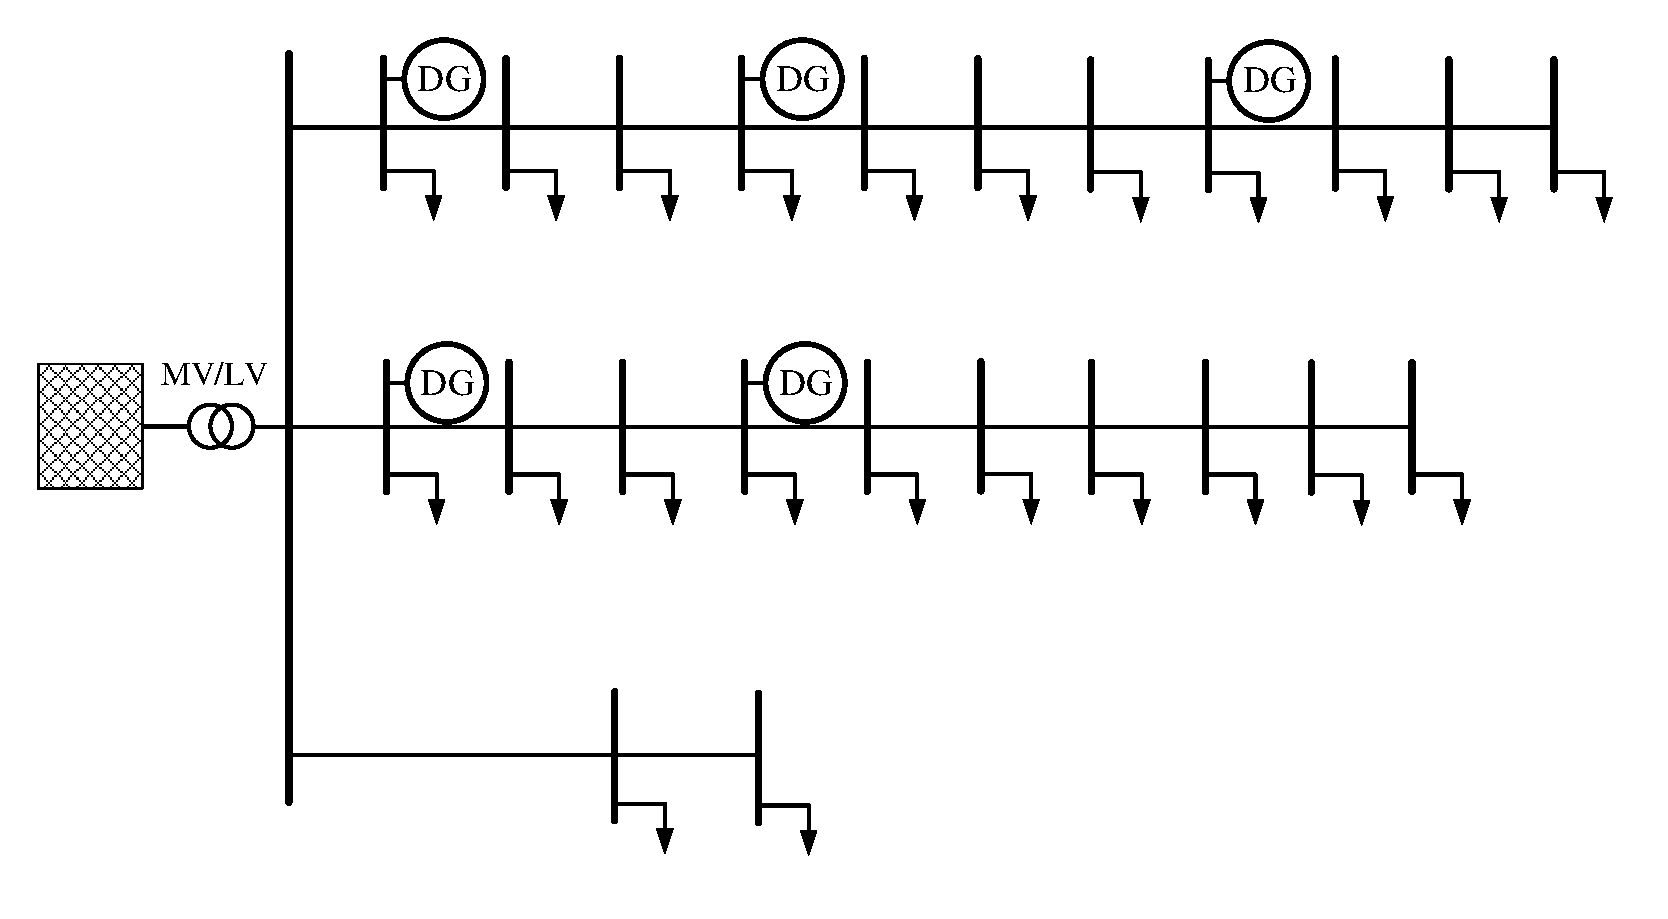
\includegraphics[width=1\columnwidth ]{ChapterOPF_DSO/Figures/LV_network_2.pdf}
	   %\vspace*{-8cm}
		\caption{LV Network scheme}
	\label{fig:case_study_LV}  
\end{figure}

The main goal of the case study is to simulate active network management for a safe distribution network operation, calculating the flexibility request to avoid network reconfiguration and congestions problems such as overloads and voltage deviations. The associated flexibility activation costs are based on the costs of demand-response activation and its impact on grid reinforcement obtained from \cite{EUCommision-DGEnergy2016, Saygn2019}. The case study implements the previously defined mathematical formulation under the LV network detailed above, and also considers the following restrictions for a correct operation, based on the operational guidelines \cite{BAYER2020336, Giannelos2016}: 

\begin{enumerate}
\item All bus voltages have to be within $\pm 3$ \% of the rated voltage, 1.01 pu.
\item All lines have a maximum loading percentage of 70 \%. 
\end{enumerate}

At these time periods where the operation constraints are not fulfilled, a congestion problem is detected, being characterized under overload, overvoltage or undervoltage, and the AC-OPF computes the flexibility requested to return the distribution network to a status where the restrictions are met again at all buses, transformers, and lines. The problem is based on a day-ahead time horizon, split into hourly time periods. The following sections cover a detailed analysis of the results under a single period, being understood as one hour, while the latter covers the operation results under a multiperiod optimization for a day-ahead scenario.  

\section{Results}
The results of the flexibility request under certain scenarios are detailed in this section. The defined scenario considers an increase of the residental load in some of the nodes, and a surplus of DERs generation in some of the nodes. The results section is structured into two main subsections, first for detailing the specific results under a single period of study (e.g 1 hour), whereas the second section draws the results for a day-ahead simulation, split into hourly time periods. While the single period section aims to detail the effect of the flexibility request under a specific time period, the day-ahead or multiperiod section aims to detail the evolution of the flexibility requests for a given day and a given scenario of load and generation profiles in the LV network. 
\subsection{Single period}
The congestion caused by a high load scenario in node 10 is an overload of line 6-10, as shown in Figure \ref{fig:congestion_pq_pre}. After the flexibility-based AC-OPF calculation, the flexibility requests are located in two different nodes, requesting both flexibility upwards and downwards for active, and reactive power flexibility, as shown in Table \ref{tab:FR_case1}. For the sake of simplicity of the results explanation, the variables related to flexibility request $\phi_{i,t}^{P^{UP}},\phi_{i,t}^{P^{DOWN}}$ and $,\phi_{i,t}^{Q}$ are represented in the following tables as $\phi_{i,t}^{P}$; represented by positive values for $\phi_{i,t}^{P^{UP}}$, negative values for $\phi_{i,t}^{P^{DOWN}}$. In the case of $\phi_{i,t}^{Q}$, this variable can take either positive or negative values depending on the type of reactive power requested, inductive or capacitive. The network status after activating the flexibility requested is shown in Figure \ref{fig:congestion_pq_post}.

\begin{table}[htbp]
\centering
\caption{Flexibility request values under a single congestion in the distribution network}
\label{tab:FR_case1}
\begin{tabular}{lll} 
\toprule
Node & $\phi_{i,t}^{P}$ [kW] & $\phi_{i,t}^{Q}$ [kvar]  \\ 
\hline
5    & 57.84      & 23.72         \\
4    & - 0.7      & - 0.2         \\
\bottomrule
\end{tabular}
\end{table}

\begin{figure}[htbp]
\centering     %%% not \center
\subfigure[Network status before the flexibility request activation]{\label{fig:congestion_pq_pre}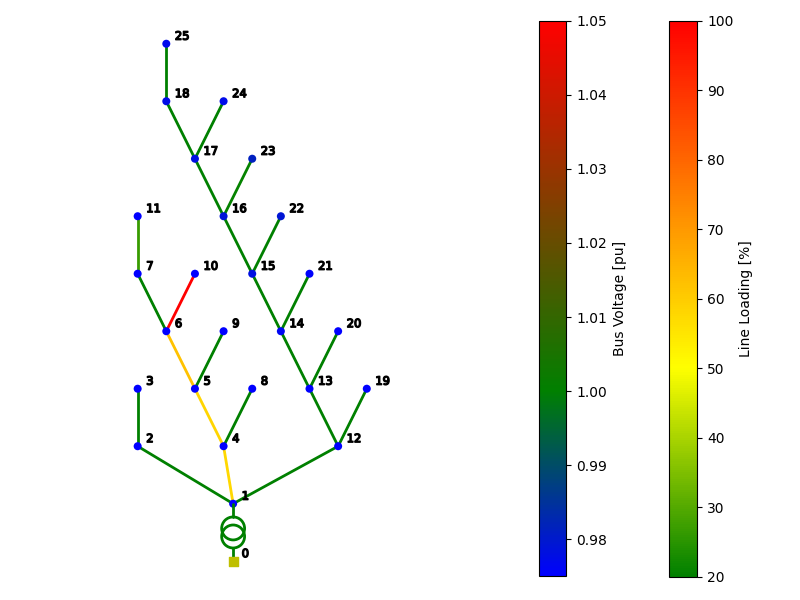
\includegraphics[width=90mm]{ChapterOPF_DSO/Figures/congestion_pq_pre.png}}
\subfigure[Network status after flexibility request being activated]{\label{fig:congestion_pq_post}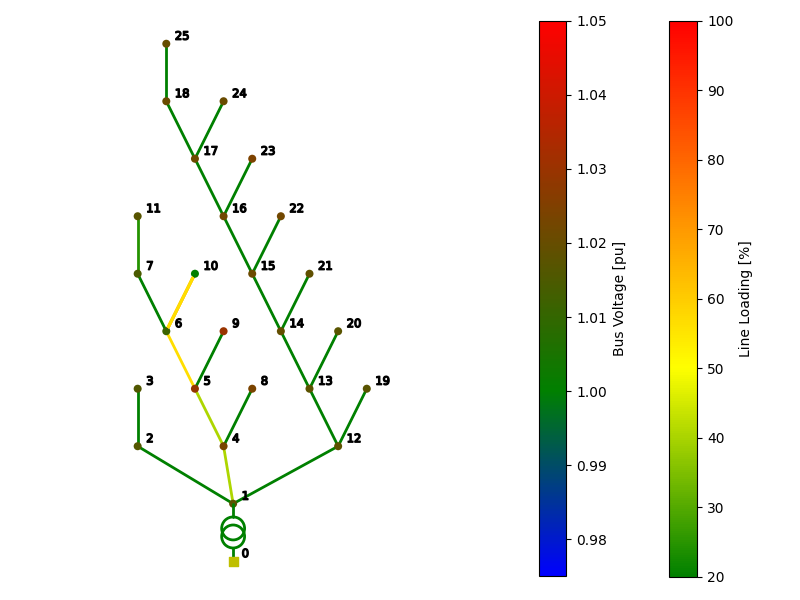
\includegraphics[width=90mm]{ChapterOPF_DSO/Figures/congestion_pq_post_2.png}}
\caption{Flexibility AC-OPF results comparison}
\label{fig:case1_fr}
\end{figure}


\begin{figure}[htbp]
\centering     %%% not \center
\subfigure[Network status before the flexibility request activation]{\label{fig:congestion_pq_pre_2points}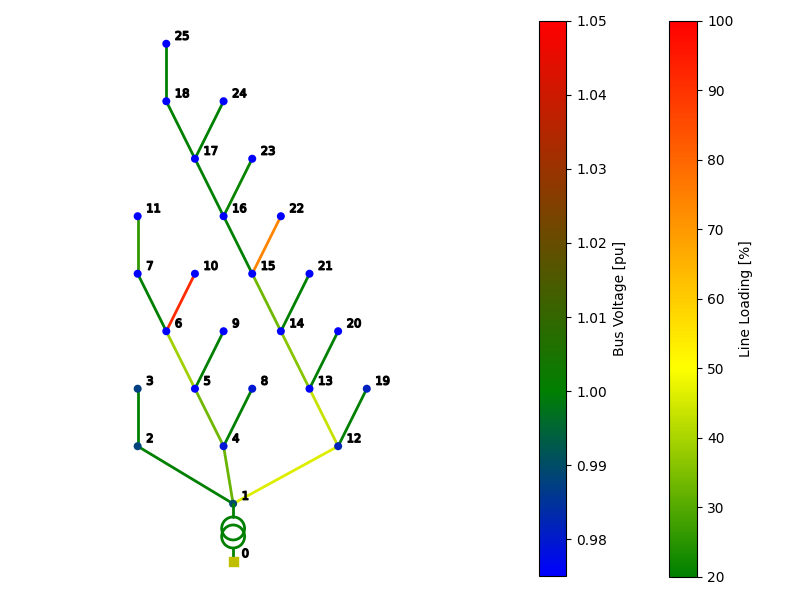
\includegraphics[width=90mm]{ChapterOPF_DSO/Figures/congestion_two_points_pre.png}}
\subfigure[Network status after flexibility request being activated]{\label{fig:congestion_pq_post_2points}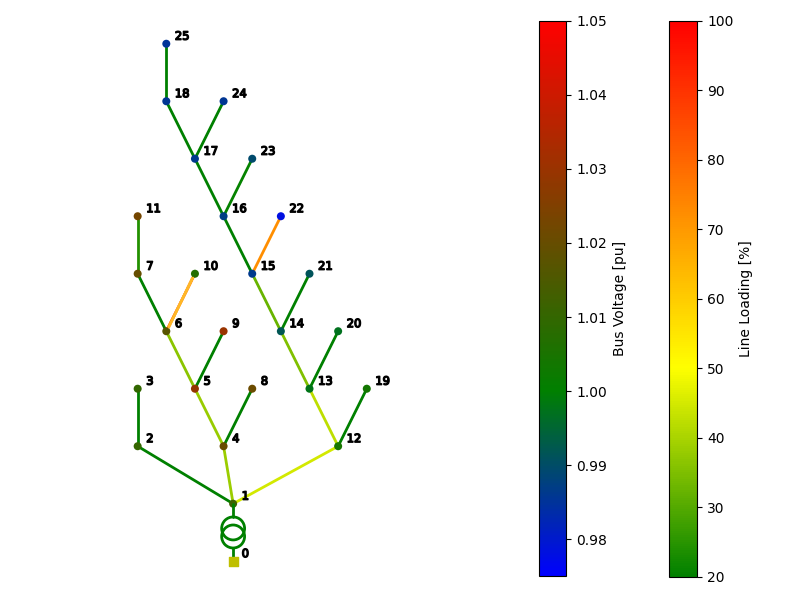
\includegraphics[width=90mm]{ChapterOPF_DSO/Figures/congestion_two_points_post_2.png}}
\caption{Flexibility AC-OPF results comparison for two identified congestions}
\label{fig:case2_fr}
\end{figure}


\subsubsection{Results for two congestions and two flexibility points}

In this second scenario, two congestions were identified on the network, one caused by a surplus of generation, and the other by an increase of the demand in one of the network nodes. In this case, congestions were characterized as overcurrent in line 8 (Nodes 6-10) with a load percentage of 91.5 \%, and in line 20 (Nodes 15-22), with a load percentage of 73.75\% (Figure \ref{fig:congestion_pq_pre_2points}). After computing the AC-OPF algorithm, flexibility is requested in three nodes, for both active and reactive power, as shown in Table \ref{tab:FR_case2}

\begin{table}[htbp]
\centering
\caption{Flexibility request values under multiple congestions in the distribution network}
\label{tab:FR_case2}
\begin{tabular}{lll} 
\toprule
Node & $\phi_{i,t}^{P}$ [kW] & $\phi_{i,t}^{Q}$ [kvar]  \\ 
\hline
5    & 17.54      & 1.99         \\
15    & 17.12      & 1.78          \\
4    & - 4.82      & - 0.29         \\
\bottomrule
\end{tabular}
\end{table}

By activating these flexibility requests, a new network status is achieved and validated by the Power Flow check at the end of the algorithm. As can be observed in Figure \ref{fig:case2_fr}, the previous network status with the indentified congestions showed that there are two lines with the loading percentage over the constraint of 70 \% (Figure \ref{fig:congestion_pq_pre_2points}). Once flexibility is activated, Figure \ref{fig:congestion_pq_post_2points} shows that the congested lines achieve a reduction of congestion around 18~\%. In this case, a greater reduction in these lines lead to a congestion located in other lines of the network, and hence to an infeasibility of the AC-OPF algorithm. 


It is important to notice that are some network buses and network scenarios where a congestion cannot be completely avoided by activating flexibility, without creating a congestion in a different location of the same network. In this case, the objective is to decrease the overload or the overvoltage problem closer to the maximum operation constraints while ensuring the AC power flow equations are satisfied at any point. In all cases, though, the AC-OPF algorithm considers a maximum line overload of 70 \%, and the voltage magnitude within the $\pm$ 3 \% of the rated voltage. 

\subsection{Multiperiod flexibility request}
This section presents a time series simulation for evaluating the formulation and the flexibility request approach under a day-ahead scenario, where the DSO knows the load forecast and can calculate the flexibility request needed for operating the grid correctly. The time series load and generation profiles are shown in Figure \ref{fig:data_opf_multiperiod}. The goal is to operate the grid under the same constraints for a single period, but calculating the flexibility requests at each time period considering the load and generation for that specific time period. 

\begin{figure}[H]
	\centering
	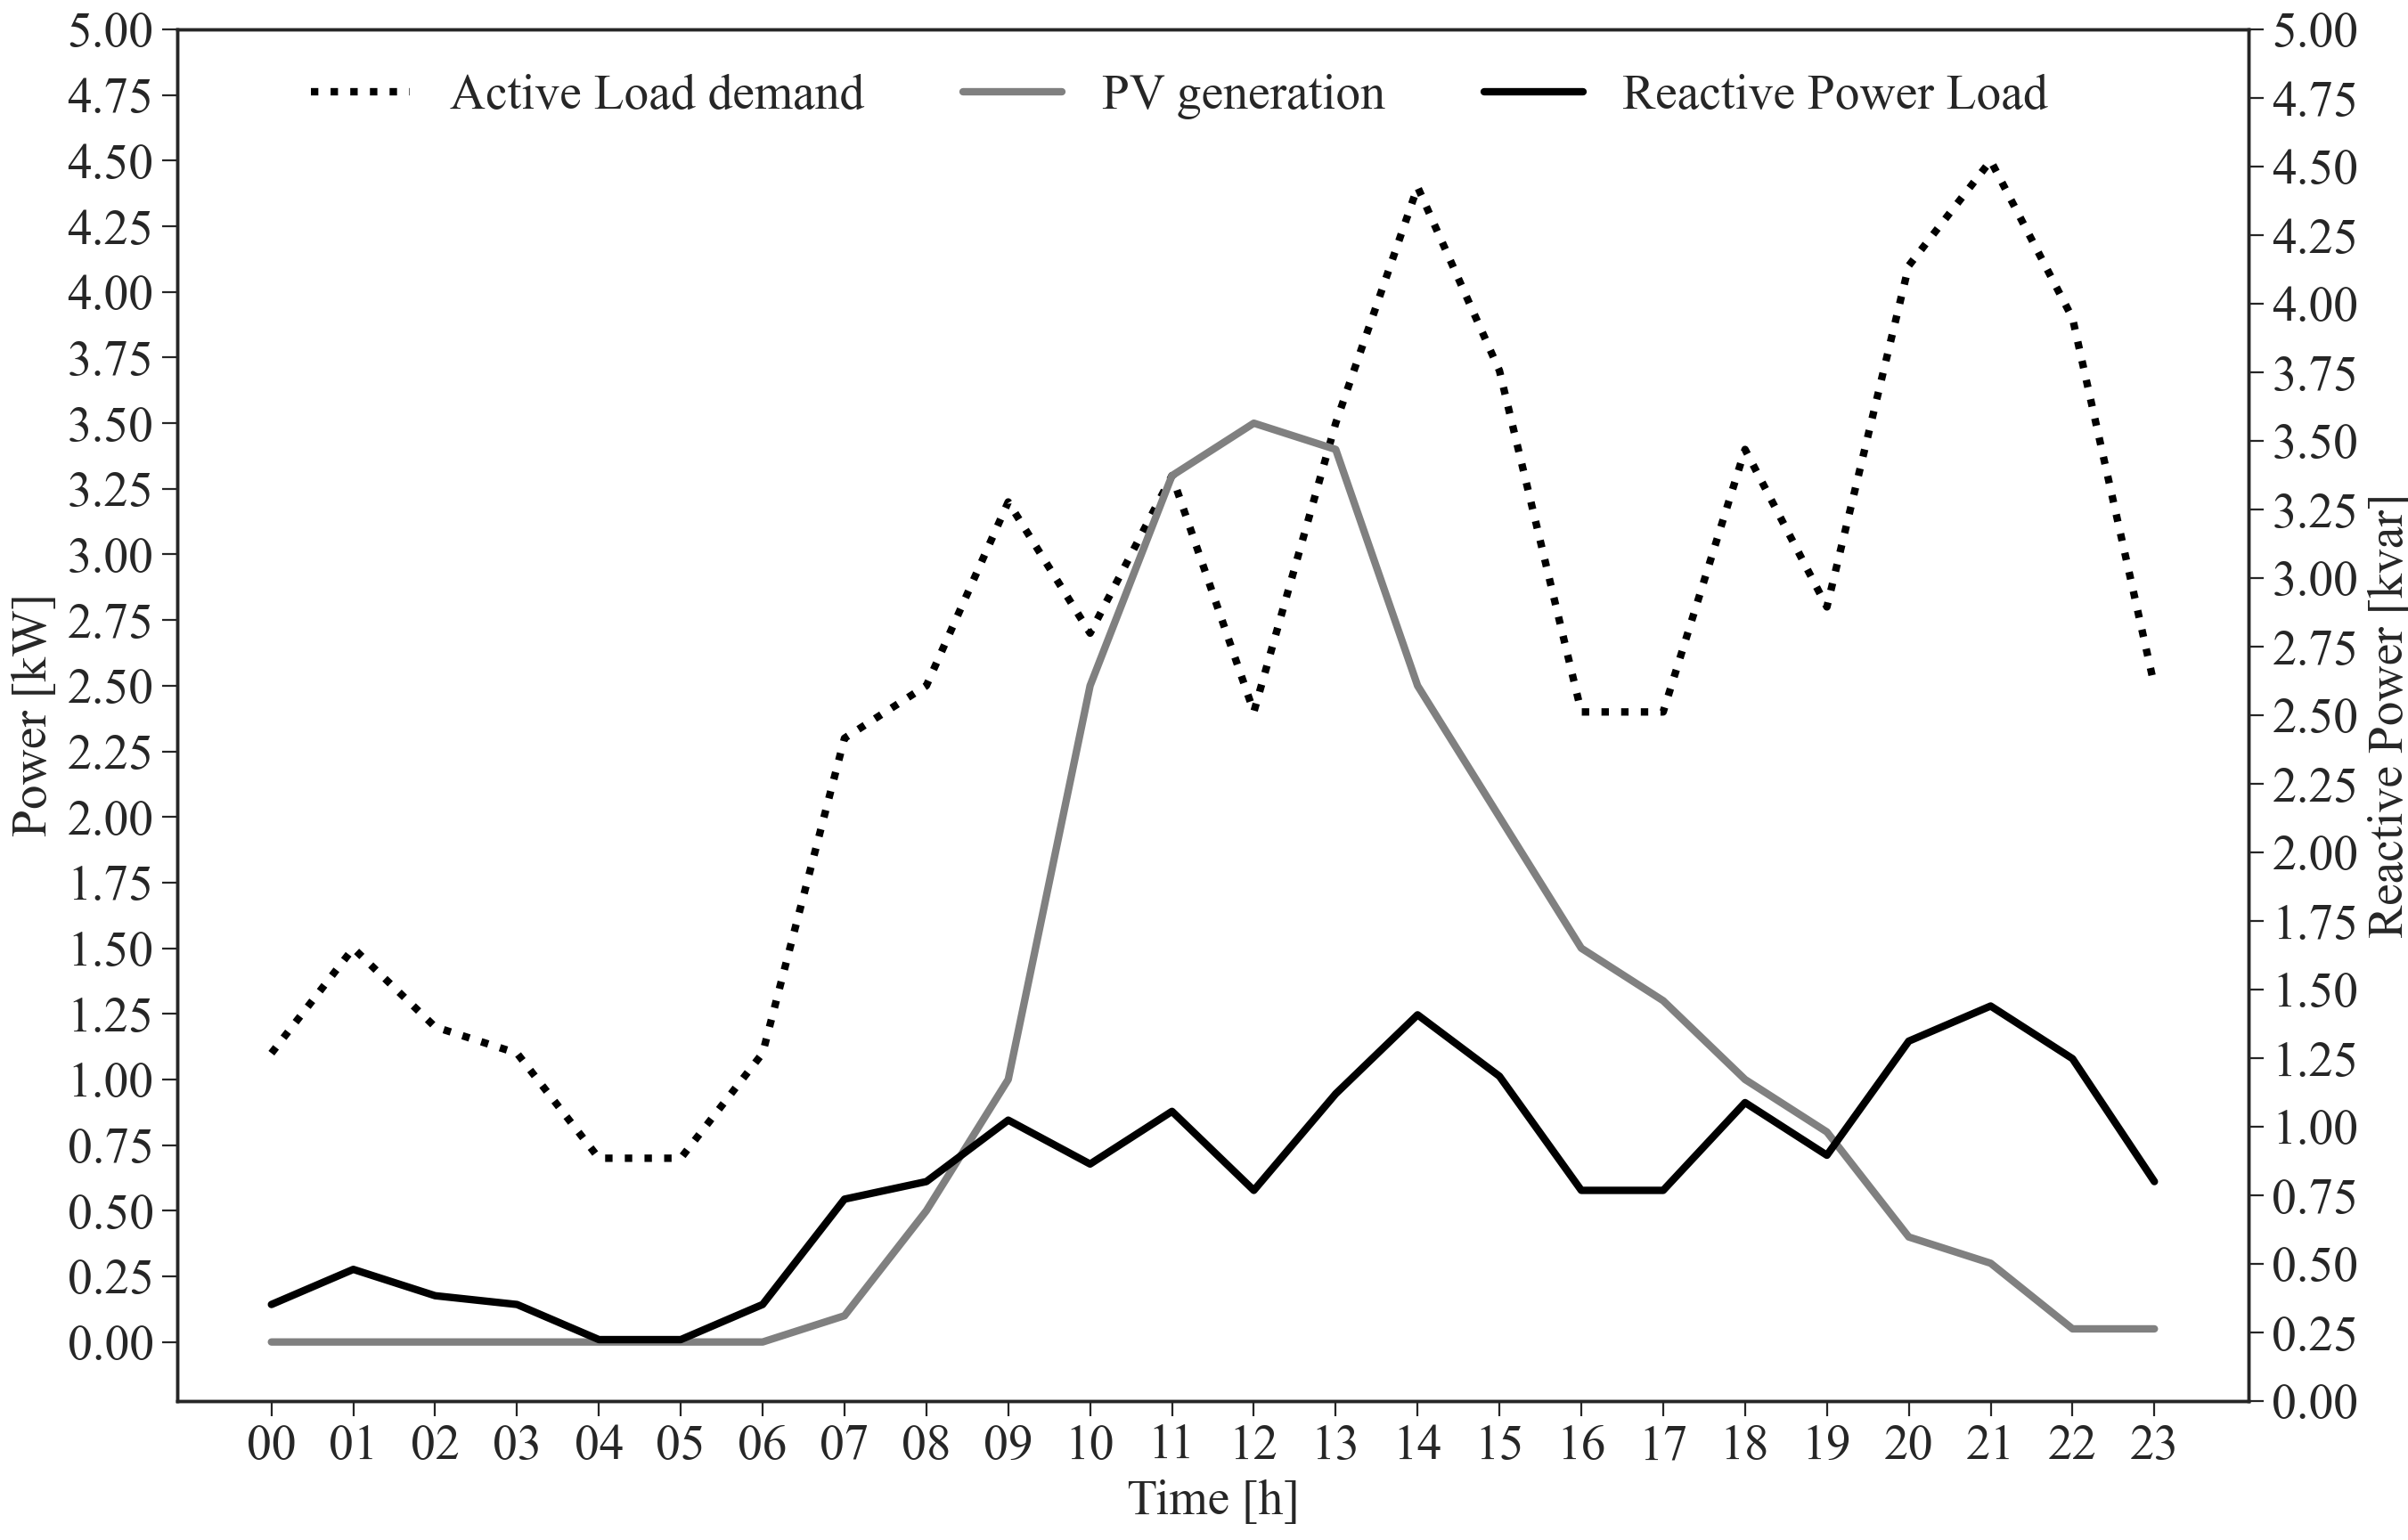
\includegraphics[width=0.8\columnwidth ]{ChapterOPF_DSO/Figures/p_q_profile_2.png}
	   %\vspace*{-8cm}
		\caption{Time-series power profiles for node 9 of the LV network}
	\label{fig:data_opf_multiperiod}  
\end{figure}

Figure \ref{fig:flex_requests} shows the flexibility requested at specific nodes of the LV network. For a better understanding of the results, only the nodes where flexibility has been requested are shown in the figures. The most congested nodes have been nodes 6, 10, 15 and 22, with overcurrents in the lines between them, and undervoltages at the end of the line. After the execution of the flexibility-based AC-OPF, flexibility is requested in nodes 4, 5 and 22, with request values between 0.5 to 57.84 kW. In any case, upward flexibility requests have always been greater than downwards flexibility requests. This can be explained because in these nodes the most common congestion detected has been undervoltage. Hence, upward flexibility provides active power in that node, and raises the voltage magnitude solving the congestion at that specific node. In a smaller scale, reactive power is requested as well in one of the network nodes. 

\begin{figure}[htbp]
	\centering
	\includegraphics[width=0.8\columnwidth ]{ChapterOPF_DSO/Figures/flex_requests_vfin.png}
	\caption{Flexibility requests for 24 time periods simulation}
	\label{fig:flex_requests}  
\end{figure}

The main objective of the flexibility request optimization problem is to find a solution where there is a local flexibility activated in one of the network nodes, reducing or mitigating the problem detected of undervoltage, overvoltage or line overload while not creating another congestion in a different network area. 
The results of the optimization problem are checked by means of the power flow equations, to check the new status of the network after finding an optimal solution. As can be seen in Figure \ref{fig:line_load}, the network lines are below the operational load percentage limit of 70\% in all time periods. There are specific time periods, being for example at 8:00 and 18:00 for line 5-4, and at 13:00 for line 14-15 where the line is operating at the upper boundary of the line load constraint. Under these periods, other feasible solutions could not be found to reduce the congestion at these lines without leading to another congestion in the lines close to these nodes involved. 

\begin{figure}[htbp]
	\centering
	\includegraphics[width=0.8\columnwidth ]{ChapterOPF_DSO/Figures/line_load_2.png}
	\caption{Line loading percentage throughout the multiperiod simulation}
	\label{fig:line_load}  
\end{figure}

This correct operation of the network can also be checked by means of the voltage magnitudes where there was a flexibility request activated or a congestion in the network. Figure \ref{fig:voltage_magnitudes} depicts the voltage magnitudes at each time period of the day-ahead simulation. As  can be seen in that figure, the operational constraint that the voltage magnitude should always be between $\pm$ 3 \% of the rated voltage (1.01 pu) is always satisfied.
 
\begin{figure}[htbp]
	\centering
	\includegraphics[width=0.8\columnwidth ]{ChapterOPF_DSO/Figures/voltage_pu_nodes_2.png}
	\caption{Voltage magnitudes in network nodes}
	\label{fig:voltage_magnitudes}  
\end{figure}

Only a single period with overvoltage was detected in the day-ahead simulation due to a large power generation by the distributed generation source. However, the most common problems detected under the multiperiod simulation have been line overloads due to significant demand in some network buses and undervoltages related to overload problems. Due to an overload of the line, voltage magnitude at the end of the congested line can drop, leading to an undervoltage. Hence, sometimes to avoid an undervoltage problem at the end of the line, an overload or overvoltage could happen. This is why flexibility activation in some specific buses can help prevent or mitigate these scenarios. 

To sum up, some considerations must be made about the mathematical formulation and the solvability of the problem. While AC-OPF has the advantage that it considers the full AC power flow equations, being the best choice for optimization of control and operation actions, it has some challenges and disadvantages that have been faced in this chapter. AC-OPF is computationally expensive and troublesome for extensive networks. In some cases, the current and available solvers such as the interior point (ipopt) or knitro used in this formulation could not obtain a solution for the case study. That means that some efforts have to be made to decrease computation time and resources to avoid the infeasibility of the solution. One option has been to change the control variables' initial values to start the simulation with a power flow feasible solution. Despite this, this is not always possible when considering power system networks. Another option could be to use the DC approximation. However, DC approximations are more suitable for transmission systems, not being possible to represent the correct behavior of a distribution network because of the impedance associated with short lines as the ones in distribution networks. 

Furthermore, in its original form, as the one being formulated in this chapter, the AC-OPF formulation is a non-linear and hence a non-convex problem. Further research on this topic should focus on deriving convex relaxations into the problem to transform the OPF problem into a convex Semi-Definite Program (SDP). Under certain conditions, that can lead to obtaining a solution that is the global optimum to the original OPF problem, achieving a zero-duality gap. If this cannot be achieved, a convex relaxation could help determine the distance between solutions.  

\section{Chapter remarks}
This chapter aimed to evaluate the possibility of defining a model for calculating the flexibility requests under a distribution network to create a tool for DSO to know in advance the flexibility required for a correct active network operation. In recent years, electricity consumption is increasing faster than it could have been expected, and the distribution network is allocating more loads, more distributed generation, and controllable assets, creating a space for prosumers. However, the network is facing operational challenges. The DSO can operate the network without reconfiguring the network or reinforcing the network through the flexibility request calculation.

Flexibility can be a valuable tool for DSOs while providing them with more knowledge about the distribution network and using demand-side flexibility to operate the grid correctly. A mathematical formulation has confirmed this hypothesis considering the flexibility activation costs and the network constraints under the AC power flow formulation. Under the case study considered, a single period and a multiperiod simulation has been carried out. In both cases, some lines and nodes were more likely to experience congestions than others, based on the characteristics of the line components and the network layout. In all cases, active power has been the main request to solve congestions in the distribution network case study. In further studies, DSOs could base their active network management on requesting active power flexibility and let the reactive power request be provided automatically by distributed generators.  

Furthermore, computational resources should be considered when evaluating more extensive distribution networks because it can compromise finding an optimal solution or the problem to converge. In these cases, either splitting the network into different feeders, using other non-linear solvers, or extracting the convex relaxation problem could help the solvability of the problem. With the objective of providing a more specific cost optimization objective function, a particular model of the flexibility activation costs should be developed to evaluate the benefits of activating flexibility compared to grid reinforcement. 

To conclude, the flexibility-based AC-OPF formulation presented in this chapter can become a standard tool for DSOs to develop active network management based on demand-side assets, being the last element in the flexibility chain constituted by end-users, aggregators, and finally distribution network operators. 